\documentclass[colorlinks]{thesis-ekf}
\usepackage[T1]{fontenc}
\usepackage[utf8]{inputenc}
\PassOptionsToPackage{defaults=hu-min}{magyar.ldf}
\usepackage[magyar]{babel}
\usepackage{graphicx,amsmath,amssymb,amsthm}
\graphicspath{{./figures/}} % A képfájlokat a [figures] mappába kell tenni!
\footnotestyle{rule=fourth}

\newtheorem{tetel}{Tétel}[chapter]
\newtheorem{lemma}[tetel]{Lemma}
\theoremstyle{definition}
\newtheorem{definicio}[tetel]{Definíció}
\newtheorem{feladat}[tetel]{Feladat}
\theoremstyle{remark}
\newtheorem{megjegyzes}[tetel]{Megjegyzés}
\newtheorem*{megoldas}{Megoldás}

\begin{document}
\logo{
\includegraphics[width=9cm]{eke-logo}}
\institute{Matematikai és Informatikai Intézet}
\title{Chemist \\ Kémiai Legó}
\author{Fehér Rózsa Zsuzsanna\\ Programtervező Informatikus Bsc}
\supervisor{Troll Ede \\Tanársegéd}

\city{Eger}
\date{2019}
\maketitle
\tableofcontents

\chapter{Bevezetés}
Szakdolgozatom témája egy Unity-ban megírt háromdimenziós ismeretterjesztő játék, ahol a Mengyelejev tábla elemei közül különféle atomokat kiválasztva molekulákat, ionokat és fémes kötéseket hozhatunk létre.
A játék célkorosztálya első sorban az általános iskolások korcsoportja. Így főként ezekben az időkben tanult kémiai kötések, atomok és molekulák felépítését szemlélteti a játék a modelleken keresztül.

A szoftver alapvetően drag and drop technológián alapul, ezért is, illetve, mert a játékfelületen törölni és mozgatni lehet a molekulákat és atomokat javasolt az egér használata.

Választásom azért esett erre a témára, mivel jómagam is nehezen tudtam elképzelni ezeket kötéseket általános iskolásként, valamint érdekelt a háromdimenziós modellezés és játékfejlesztés is. Így a Unity-vel lehetőségem volt közelebbről megismerkedni a játékfejlesztéssel magával, illetve a modellezés lépéseivel, valamint a kémiai háttér tudásom is gyarapodott.

A szakdolgozat részletezni fogja a technológiát, illetve összehasonlítja más fejlesztőkörnyezetekkel. Ismertetni fogja, hogy milyen kémiai ismeret volt szükséges a szoftver elkészítéséhez, valamint bemutatásra kerül maga a játék is az azokban használt modellekkel, és felhasználói interakció lehetőségekkel együtt. 

Mivel a témakör elég tág, illetve az oktató játék csak szűkös tudományos forrással készült, ezért a továbbfejlesztési lehetőségek akár több irányban is folytatódhatnak.

\chapter{Kémia az iskolákban}

min 2 oldal

\chapter{Kémiai háttér}

A játék működéséhez elengedhetetlen az atom felépítésének és a kötések kialakulásának ismerete. 
\section{Atomok}

Mint tudjuk az atomok protonokból, neutronokból és elektronokból állnak. A protonok töltése pozitív, az elektronoké negatív, a neutronok töltését pedig tekintsük szemlegesnek. Az elektronokon kívül a nukleonok az atom magjában található, míg az elektronok az atom mag körül ''keringenek,, előre meghatározott
elektronpályákon. 

Mivel az atomok szabad állapotban a természetben ritkán fordulnak elő (kivéve a nemesgázok stabil szerkezetük miatt), fontos a kémia kötésekről beszélnünk, ugyanis csak is ezek a reakciók teszik lehetővé azt, hogy a periódusos rendszerbeli elemek elérjék a kívánt stabil(nemesgázbeli) állapotukat. Ezt úgy teszik, hogy más atomokkal különböző kötéseket létesítenek.\cite{ionos_vidi} De mégis mi határozza meg azt, hogy milyen kötés alakul ki két szabad atom között?

Az atomokban és molekulákban lévő elektronok elhelyezkedése, azaz az elektronszerkezet, határozza meg az atomok és molekulák kémiai viselkedését.\cite{wiki_e_szerk}
Azokat az anyagokat, amik ugyanolyan rendszámú (azaz azonos mennyiségű elektronnal rendelkező) atomokból épülnek fel, kémiai elemeknek hívjuk, és vegyjellel hivatkozunk rájuk.\cite{periodusos_ppt} 

A későbbiek folyamán az atom megnevezést a kémiai elemekre fogom használni. A szoftver szempontjából a kettőt egyformának tekinthetjük.

Az elektronszerkezeten belül, az elektronkonfiguráció, és azon belül a legkülső héj elektronkonfigurációja valamint az ahhoz kapcsolódó vegyérték elektronok, illetve az elektronegativitás játszik szerepet abban, hogy egy atom milyen kötést tud létesíteni más atomokkal. 

Kémiai kötésnek nevezzük azt, amikor több atom reakcióba lépése során egy közös, stabil (telített) külső elektronhéj alakul ki.Ezek lehetnek elsőrendű és másodrendű kémiai kötések. A kovalens, ionos és fémes kötés az elsőrendű kötések közzé tartozik\cite{miskolc_kemia}, valamint a játék is csak ezekkel a kötésekkel foglalkozik.

Az elektronkonfiguráció az elektronok pályák szerinti elrendeződését írja le egy atomban.\cite{periodusos_ppt} Mivel az elektronpályák nem expliciten töltődnek fel, hanem az al héjak energiaszintjének megfelelően, így sokszor előfordul, hogy egy elektronpálya (elektronhéj) még nem telítődik meg, de már az eggyel nagyobb héjon észlelhetünk elektronokat.
A legkülső elektronhéjat szokás vegyértékhéjnak nevezni, míg az ezen tartózkodó elektronokat vegyértékelektronoknak\cite{vegyérték_sulinet} Ezek közül kerülnek i azok az elektronok amik képesek kötéseket kialakítani (vegyértékeke), illetve ionos kötésnél a vegyérték elektronok száma határozza meg azt, hogy ők adják-e át a másik atomnak az elektronjaikat, vagy ők veszik el.\cite{ionos_vidi}

Az elektronegativitás(EN) olyan mennyiség, ami azt írja le, hogy mekkora elektrosztatikus erő hat a másik atom vegyértékelektronjaira.\cite{angol_en} Értékét Slater szabállyal, illetve az empirikus megfigyeléseken alapuló Pauli elektronegativitási rendszerrel lehet meghatározni. Utóbbiban az atomokhoz tartozó elektronegativitásokat a lítiumhoz és fluorhoz képest viszonyították. Mivel viszonyszám, mértékegysége nincs.\cite{miskolc_kemia}\cite{eke_kemia_ppt}

\begin{figure}[!ht]
	\centering
	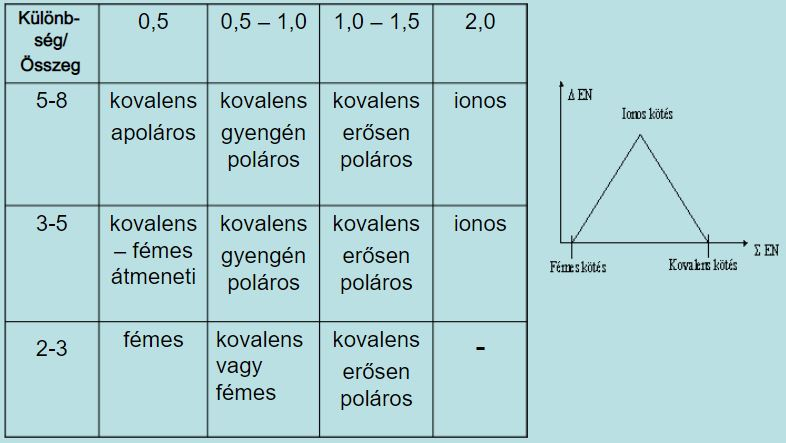
\includegraphics[width=9cm]{en_slide}
	\caption{\cite[52.~ppt]{periodusos_ppt}}\label{EN_tablazat}
\end{figure}
\Aref{EN_tablazat} látható, hogy milyen kötések alakulhatnak ki az elektronegativitástól függően, ahol a \begin{math}\Delta EN\end{math} a két atom elektronegativitásai között különbséget, míg \begin{math}\Sigma EN\end{math} az összeget jelöli.\cite{eke_kemia_ppt}
\section{Ionos kötés}

Ionos kötésnél két ionizált atom között lép fel elektrosztatikus vonzás.
Atomból ion úgy alakulhat ki, hogy az atommal közölnek egy bizonyos mennyiségű energiát. Ez az ionizációs energia. 

Definíció szerint az ionizációs energia, nem más, mint az az energiamennyiség  amely az n-edik elektron leszakításához szükséges, miután az előző n–1-et már leszakítottuk.\cite{miskolc_kemia}
Ilyenkor a nagyobb elektronegativitással rendelkező ion elektronokat vesz el a kisebb elektronegativitású atom vegyértékelektron héjáról, viszont a két atom teljes egybeolvadását az alacsonyabb elektronhéjak taszító hatása megakadályozza.\cite{miskolc_kemia}

Az, hogy hány elektront tud leszakítani, illetve hányat képes befogadni az ion attól függ, hogy milyen messze van a nemesgáz konfigurációtól.

Nemesgáz konfiguráció alatt az értjük, amikor az elektronszerkezet a legstabilabb. Gyakorlatban ez azt jelenti, hogy a vegyértékhéjon nyolc vegyérték elektron van, azaz telítve van az al héj.\cite{ionos_vidi}

Tehát ha vennénk két atomot,melyeknek elektronegativitásuk közötti különbség legalább kettő (Lásd \aref{EN_tablazat}.~ábra), akkor az egyik atommagja elkezdi vonzani a másik atom elektronjait, és ugyanezt teszi a másik is, így közeledve egymáshoz. Végül a nagyobb \begin{math} EN\end{math}-el rendelkező atom húzná el a másik vegyérték elektronjait. De abból is csak annyit, hogy ő maga, illetve a másik atom is nemesgáz konfigurációba kerüljön. \cite{ionos_vidi}
\section{Fémes kötés}


\section{Kovalens kötés}
 A maximális vegyérték egy oszlopon belül változhat. A felsőbb periódusokban az elemek rendszerint kevesebb vegyértékelektronnal képesek kötést létesíteni, mint az alsóbb periódusokban található elemek.\cite{periodusos_ppt}
\chapter{Unity és a fejlesztői lehetőségek}
min 2 oldal
\chapter{Chemist}
\section{Általános leírás}
min 2 oldal
\section{Modulok}
\subsection{Menü}
min 2 oldal
\subsection{Periódusos rendszer}
min 2 oldal
\subsection{Shader}
min 2 oldal
\subsection{Fémes és inos kötés modellje, és működése}
min 2 oldal
\subsection{Kovalens kötés}
min 2 oldal
\chapter{Továbbfejlesztési lehetőségek}
\chapter{Ábrák jegyzéke}
\begin{thebibliography}{1}
	\bibitem{wiki_e_szerk} \textsc{Wikipédia}: \url{https://hu.wikipedia.org/wiki/Elektronszerkezet} (Hozzáférés ideje: 2019.03.12).
	\bibitem{periodusos_ppt} \textsc{SlidePlayer}: \url{https://slideplayer.hu/slide/11181363/} (Hozzáférés ideje: 2019.03.12).
	\bibitem{miskolc_kemia} \url{http://web.uni-miskolc.hu/~www_fiz/majar/Oktatas/anyagmernok_levelezo/Fizika2_KemiaiKotesek.pdf} (Hozzáférés ideje: 2019.03.12).
	\bibitem{vegyérték_sulinet} \textsc{Suli Net}: \url{https://tudasbazis.sulinet.hu/hu/termeszettudomanyok/kemia/szervetlen-kemia/a-vegyertek-kapcsolata-az-elektronszerkezettel/a-vegyertek-kapcsolata-az-elektronszerkezettel} (Hozzáférés ideje: 2019.03.12).
	\bibitem{ionos_vidi} \textsc{Youtube}: \url{https://www.youtube.com/watch?v=nN7HoYkTdKk} (Hozzáférés ideje: 2019.03.12).
	\bibitem{angol_en} \url{https://chem.libretexts.org/Bookshelves/Physical_and_Theoretical_Chemistry_Textbook_Maps/Supplemental_Modules_(Physical_and_Theoretical_Chemistry)/Physical_Properties_of_Matter/Atomic_and_Molecular_Properties/Electronegativity/Allred-Rochow_Electronegativity} (Hozzáférés ideje: 2019.03.12).
	\bibitem{eke_kemia_ppt} \textsc{Eszterházy Károly Egyetem}: \url{kemia.ektf.hu/kemiai_kotesek.ppt} (Hozzáférés ideje: 2019.01.31).
\end{thebibliography}
\end{document}
